\documentclass[11pt,a4paper]{article}

\usepackage{classeRapport}

\begin{document}

\PageDeGarde	
{business-cat.jpg} % image sur la page de garde
{Modèle de rapport \LaTeX{}} % titre principal
{Pour les aventuriers\\et ceux qui n'ont pas le choix} % sous-titre
{Prénom \textsc{Nom}\\
Prénom \textsc{Nom}\\
Prénom \textsc{Nom}} % nom
{Module – Département – Année} % bas de page


\Page{INSALogo} % logo de bas de page (en bas a droite)

\tableofcontents

\clearpage % Pour faire un saut de page propre
\section*{Introduction} % L'astérisque est pour que la section ne soit pas numérotée
\addcontentsline{tod}{section}{Introduction} % Cette commande ajoute la section à la table des matières malgré le fait qu'elle ne soit pas numérotée

    Ce document a pour but de fournir une base aux étudiants souhaitant rédiger un rapport en \LaTeX.
    Il a été conçu dans le but d'être utilisé pour les projets d'I4.2 mais peut très facilement être réutilisé pour d'autres projets, que ce soit en STPI ou en département.
    Il n'a pas vocation à être exhaustif sur comment utiliser le \LaTeX{} pour écrire un rapport, mais tente de donner suffisamment de ressources pour que des étudiants curieux et débrouillards puissent s'en sortir sans trop d'égratignures.


\clearpage % Pour faire un saut de page propre

\section{Analyse du projet}
Il est probable que vous n'ayez pas besoin d'une autre section dans votre document.
Vous pouvez donc supprimer celle-ci faire remonter toutes les sous-sections et sous-sous-sections d'un cran.
    
    \subsection{Cahier des charges}
        \subsubsection{Description du projet}
            Le groupe a décidé de faire un projet de snake en I4.2 par ce qu'on a pas le choix de faire autre chose.
            Le snake est un jeu qui… blablabla à vous de faire votre description.
        \subsubsection{Liste des fonctionnalités}\label{sssect:fonctionnalites}
            Le rendu final de notre projet comportera les fonctionnalités suivantes:
            \begin{itemize}
                \item Affichage console
                \item Choix de la taille du plateau
                \item Choix de la difficulté
                \item …
            \end{itemize}
            
            Nous avons prévu des fonctionnalités optionnelles, qui ne seront implémentées que s'il nous reste du temps à la fin du semestre:
            \begin{itemize}
                \item Coloration de l'affichage
                \item Jeu multijoueur
                \item Sauvegarde des scores
                \item …
            \end{itemize}
            
            Versions prévues:
            
            V1 (15/04/2020):
            \begin{itemize}
                \item Affichage du plateau
            \end{itemize}
            
            V2:
            \begin{itemize}
                \item …
            \end{itemize}



    \subsection{Conception globale}
        Cette section présente la conception globale du programme implémentant les fonctionnalités données en section~\ref{sssect:fonctionnalites}.
        L'analyse descendante correspondante est donnée en figure~\ref{fig:AD}.
        
        \begin{figure}[!ht]
            \centering % Centre horizontalement tout ce qui est dans l'environnement ``figure''
                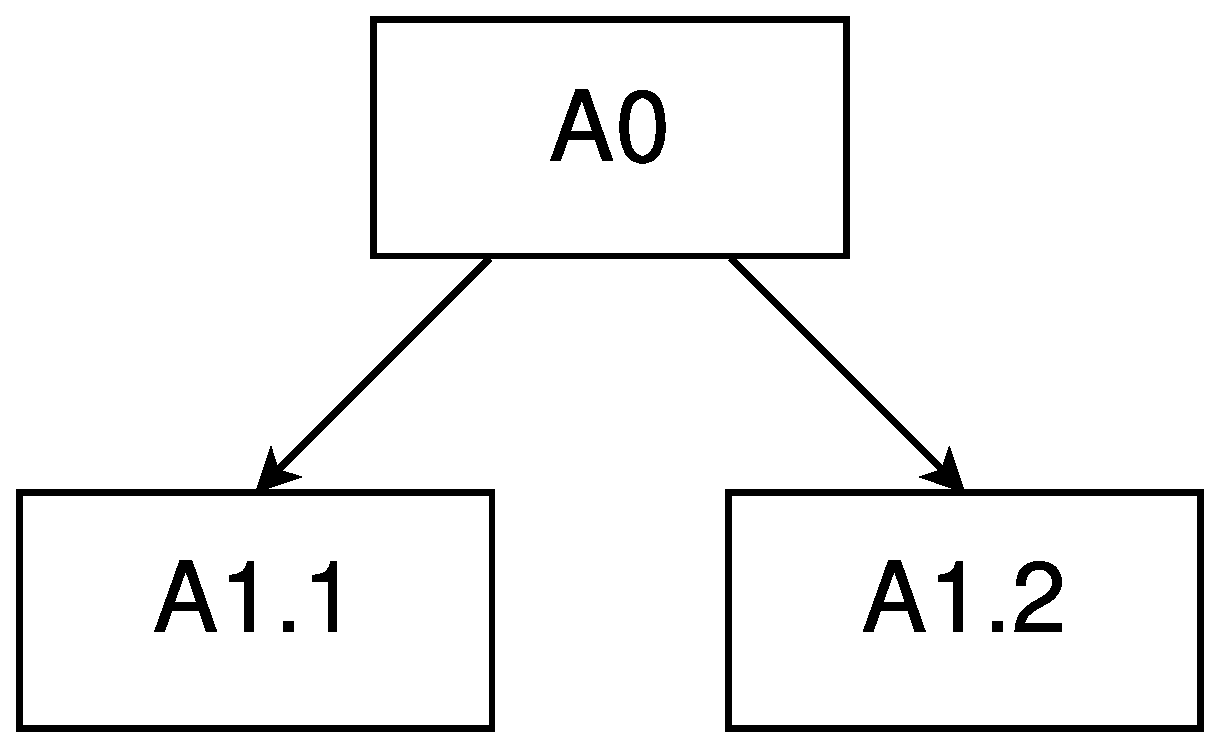
\includegraphics[width=0.5\textwidth]{images/AD.eps} % Chemin vers l'image à ajouter
            \caption{Analyse descendante du projet.} % Légende de l'image
            \label{fig:AD} % Étiquette pour y faire référence ailleurs dans le document
        \end{figure}
        
        Je vous invite à utiliser le programme dia\footnote{\url{https://fr.wikipedia.org/wiki/Dia_(logiciel)}} pour réaliser votre analyse descendante et vos autres diagrammes.
        Le format \verb|.eps| est un très bon choix pour exporter les diagrammes faits avec ce programme étant donné qu'il est vectoriel et très bien géré par \LaTeX{}.
    
    \subsection{Conception préliminaire}
        Le contenu de cette section présente la signature des fonctions et procédures de l'analyse descendante, en précisant les entrées, sorties et entrées/sorties.
        Il peut être intéressant de détailler la signature de certaines fonctions pour justifier certains de vos choix.
        
        Les types personnalisés employés doivent aussi être présentés et défendus dans cette section.
        
    \subsection{Conception détaillée}
        Pour vous aider à écrire des algorithmes propres en \LaTeX{} un paquet spécifique (\verb|algorithm2e|) a été ajouté par défaut à ce modèle de rapport.
        Il vous permet d'inclure du pseudo-code dans votre document pour détailler les algorithmes importants de votre programme.
        Voici un exemple d'un algorithme tiré du projet de morpion du cours d'I2:
        
        \begin{algorithm}[H]
            \SetAlgoLined
            \Fun{aGagne(g :  Grille): Emplacement}{
            \Sortie{s'il n'y a aucun gagnant, l'emplacement renvoyé est l'emplacement vide (\_), sinon c'est l'emplacement représentant la couleur du gagnant (X ou O).}
            \Donnees{i, j: Entier, vainqueur: Emplacement}
            
            vainqueur $\leftarrow$ \_\;
            
            \tcp{lignes}
            \Pour{i $\leftarrow$ 1 à 3}{
                \Si{(g[i][1] = g[i][2]) et (g[i][1] = g[i][3])}{
                    vainqueur $\leftarrow$ g[i][1]\;
                }
            }
            \tcp{colonnes}
            \Pour{j $\leftarrow$ 1 à 3}{
                \Si{(g[1][j] = g[2][j]) et (g[1][j] = g[3][j])}{
                    vainqueur $\leftarrow$ g[1][j]\;
                }
            }
            
            \tcp{diagonales}
            \Si{((g[2][2]= g[1][1]) et (g[2][2]= g[3][3])) ou\\ 
                ((g[2][2]= g[1][3]) et (g[2][2]= g[3][1]))}{
                vainqueur $\leftarrow$ g[2][2]\;
            }
            
            \Retour{vainqueur}
            
            }
            \caption{recherche d'un gagnant dans une grille de Morpion}
        \end{algorithm}
        
        Le mot-clé \enquote{\textbf{Données}} est utilisé pour déclarer les variables utilisées dans l'algorithme.
        
        La documentation du paquet \LaTeX{} pour écrire des algorithmes (\verb|algorithm2e|) est disponible à l'adresse suivante: \url{http://ctan.mines-albi.fr/macros/latex/contrib/algorithm2e/doc/algorithm2e.pdf}(voir notamment la p.41 et les suivantes pour les mots-clés a utiliser pour écrire votre algo en français).
        J'ai implémenté en plus du paquet de base les commandes \verb|\fun{}{}| pour les fonctions et \verb|\proc{}{}| pour les procédures.
        Ces commandes prennent en premier paramètre le nom de la fonction et ses paramètres et en second paramètre le corps de la fonction.
    \subsection{Implémentation}
        Il est aussi possible en \LaTeX{} d'inclure du code source dans un document.
        
        \begin{lstlisting}[language=Pascal,frame=single,caption=code source de la fonction aGagne.]
function aGagne(g :  Grille):Emplacement;
var i,j : Integer; vainqueur: Emplacement;
begin
   vainqueur := _;

   {lignes}
   for i := 1 to 3 do
   	 if (g[i][1] = g[i][2]) and (g[i][1] = g[i][3]) then 
		vainqueur := g[i][1];
	
   {colonnes}
   for j := 1 to 3 do
   	 if (g[1][j] = g[2][j]) and (g[1][j] = g[3][j]) then 
		vainqueur := g[1][j];
   
   {diagonales}   
   if ((g[2][2]= g[1][1]) and (g[2][2]= g[3][3])) or
		((g[2][2]= g[1][3]) and (g[2][2]= g[3][1])) then
			vainqueur := g[2][2];
   aGagne := vainqueur;
end;
        \end{lstlisting}

\newpage
\section{Apport du Projet}

    \subsection{Apprentissage du \LaTeX}
        Afin de réaliser notre rapport, nous avons suivi les directives données par les professeurs, à savoir utiliser le \LaTeX{}.
        
        \subsubsection{Découverte de ce langage}
            \paragraph{Site Overleaf} Nous avons fait le choix pour ce projet d'utiliser le site/application Overleaf afin de pouvoir modifier notre rapport simultanément et travailler ensemble. De plus, Overleaf permet de compiler le code directement afin d'avoir un aperçu sur la moitié de l'écran, ce qui est extrêmement pratique lorsque l'on commence à coder en \LaTeX{} car il n'est pas aisé de se représenter le rendu. Enfin, ce site fonctionne par projet, il est donc facile de partager tout le projet à son groupe et de travailler avec les mêmes fichiers indispensables tels que des images.
            
            \paragraph{Avantage du \LaTeX{}} Le \LaTeX{} a été quasiment indispensable pour la rédaction de notre cahier des charges et du rapport. Effectivement, nous avons dû insérer du code, qu'il s'agisse de pseudo-code ou de pascal, ce qui aurait été bien plus complexe avec un éditeur comme Word ou Libre office. Le \LaTeX{} permet également des rendus de qualité et il est important pour nous de découvrir ce langage.
            
            \paragraph{Les bases du \LaTeX{}} Pour la plupart des membres du groupe, nous n'avions que très peu ou jamais codé en \LaTeX{}. Ainsi, la découverte réelle de ce langage a été réalisée lors de l'élaboration du cahier des charges. Ce dernier étant assez rapide et condensé, il a permis de découvrir doucement les bases du \LaTeX{}. 

        
        \subsubsection{Approfondissement}
            \paragraph{Besoins supplémentaires} Après avoir acquis les bases indispensables à la création d'un document telles que l'ajout de titres, sections, sous-sections, paragraphes ; nous avons dû apprendre à insérer des images, des algorithmes, des parties de code. L'essentiel de cet apprentissage s'est fait grâce aux explications que l'on peut trouver sur le net. En outre, rédiger un rapport sur un seul document \LaTeX{} n'aurait pas été lisible et compréhensible, d'autant plus que nous l'avons rédigé à cinq. Organiser la rédaction du rapport s'est alors révélé très utile. Nous avons décomposé le rapport en plusieurs sections et avons fait les imports de packages dans un autre document. Cela a permis d'apporter beaucoup de lisibilité et de ne pas modifier involontairement les parties du code déjà réalisées.
            
            
            \paragraph{Difficultés rencontrées} Nous avons pu utiliser un modèle de rapport en \LaTeX{} fourni par les professeurs. Celui-ci nous a beaucoup aidé notamment pour la structure du rapport. Cependant, nous avons tout de même rencontré des difficultés comme pour importer des images, notamment l'analyse descendante qui a une taille importante, mais aussi l'insertion de code. Pour réussir à surpasser la difficulté de ce dernier point, certains membres du groupe ont appris à utiliser le package minted. 
            \newline
            De plus, nous avons rencontré de nombreuses difficultés lors de l'implémentation de notre jeu, notamment, avec l'utilisation de la SDL. En effet, dans un soucis de réalisme, pour que notre jeu soit le plus agréable possible à jouer, la gestion de l'affichage et des délais des objets de notre jeu était la partie la plus compliquée à implémenter, particulièrement lors des éboulements. De plus, il y avait beaucoup de petits détails à prendre en compte qui ne paraissaient pas très importants individuellement, mais qui, additionnés, transforment l'expérience de jeu, par exemple, le curseur quand on appuie sur échap en pleine partie, ou la gestion du chrono et des pauses quand on est dans le menu. 
                



    \subsection{Travail en groupe}
        
        \subsubsection{Découverte et utilisation de Gitlab} L'utilisation de Gitlab nous a été imposé par nos professeurs. Nous n'avions jamais utilisé Gitlab et les débuts sur ce logiciel étaient un peu compliqués, notamment pour comprendre le fonctionnement des différentes commandes. Malgré ces quelques complications, nous avons pu apprendre, à force d'utiliser les commandes, à comprendre leurs fonctions. 
        
        
        \subsubsection{Mise en accord sur les fonctionnalités} Pour les différentes fonctionnalités attendues, chacun a proposé ses idées et nous nous sommes mis d'accord pour savoir si c'était réalisable et si cela rentrait dans les fonctionnalités obligatoires ou facultatives. 
        
        
        \subsubsection{Répartition du travail en fonction des aptitudes}
        Concernant la répartition du travail au sein du groupe, nous nous sommes réparti les différentes tâches en fonction des compétences de chaque membre du groupe. Les missions principales de ce projet ont été la rédaction du cahier des charges, de l'analyse descendante et du rapport, mais aussi l'écriture du code dans le langage de programmation demandé.
        
         \subsubsection{Limitations et perspectives}
        Tout d'abord, l'aspect à distance de notre projet a rendu très difficile le travail de groupe et nous avons dû nous organiser en ligne sur Discord et Messenger. Ensuite, le suivi des séances avec le professeur était tout le temps à distance et nous n'avons pas eu de véritable retour sur notre avancée sur le projet. Enfin, concernant les perspectives, nous avions établi plusieurs fonctionnalités facultatives dans notre cahier des charges, mais que, faute de temps, nous n'avons pas mis dans notre rapport. C'est pourquoi nous voudrions les reprendre par la suite pour les intégrer dans notre Boulder Dash.
        
        


\clearpage % Pour faire un saut de page propre

\section{Conclusion}

    J'espère que ce modèle de document vous sera utile pour apprendre le \LaTeX{} et faire de beaux documents pour vos rapports, à l'INSA et ailleurs!


\clearpage % Pour faire un saut de page propre

\section*{Sources} % L'astérisque est pour que la section ne soit pas numérotée
\addcontentsline{toc}{section}{Sources} % Cette commande ajoute la section à la table des matières malgré le fait qu'elle ne soit pas numérotée
    \begin{itemize}
        \item Photo de la page de garde: \url{https://knowyourmeme.com/photos/100097-business-cat}
        \item Photo du chien page~\pageref{chien}: \url{https://knowyourmeme.com/photos/234142-i-have-no-idea-what-im-doing}
        \item Photo de lapin avec un pancake sur la tête~\pageref{lapin}: \url{https://knowyourmeme.com/photos/33054-pancake-bunny}
    \end{itemize}


\end{document}
